\newpage
\section{Automation of PML Coefficients} \label{PML-Coefficient-Automation}

Because there is a separate Perfectly Matched Layer at every boundary face of the domain (4 sides in two dimensions and 6 faces in three dimensions), it is necessary to choose the coefficients that describe the size and strength of each PML at each face. Since choosing the coefficients by relying on intuition can often result in errors, and entering them manually for each test run can be time consuming, we present an algorithm for determining the PML coefficients given the set of finite elements (triangles in two dimensions and tetrahedrons in three dimensions), as well as their individual physical characteristics ($V_p, V_s$, etc).

\subsection{What are Perfectly Matched Layers}

Perfectly Matched Layers are artificial absorbing boundary conditions for wave equations, commonly used to truncate computational regions in numerical simulations of infinite domains. It is different than typical absorbing boundary conditions in that waves originating from the non-PML region and entering PML regions do not reflect at the interface.

Perfectly Matched Layers are similar to Absorbing Boundary Conditions in that they attempt to simulate an infinite domain by absorbing the energy that reaches the boundary layers. However there are some key differences in implementation and appearance of the final image:

\begin{figure}[ht]
	\centering
	\begin{subfigure}{0.5\textwidth}
		\centering
		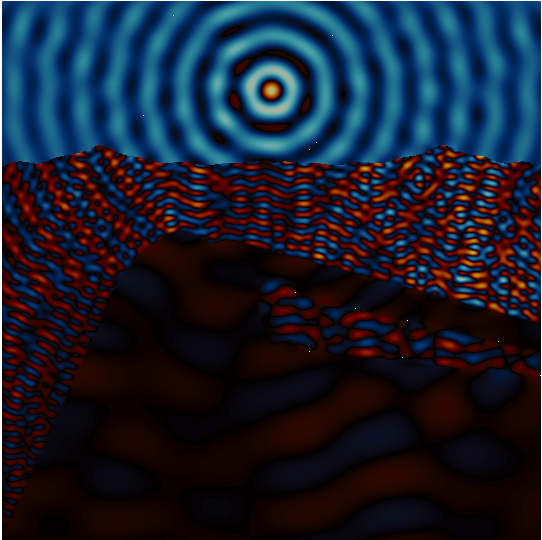
\includegraphics[width=0.8\textwidth]{Images/ABC.png}
		\caption{Absorbing Boundary Conditions}
		\label{fig:ABC}
	\end{subfigure}%
	\begin{subfigure}{0.5\textwidth}
		\centering
		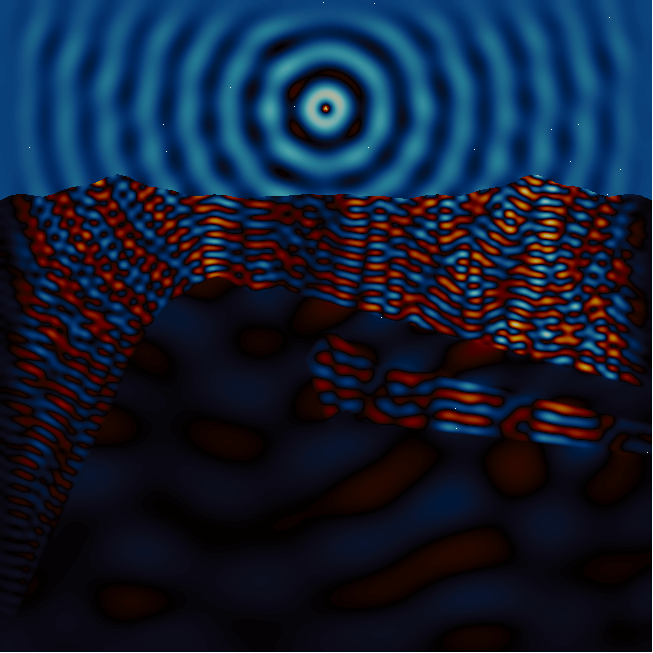
\includegraphics[width=0.8\textwidth]{Images/PML.png}
		\caption{Perfectly Matched Layers}
		\label{PML}
	\end{subfigure}
	\caption{Left: Absorbing Boundary Conditions. Right: Perfectly Matched Layers}
	\label{fig:ABC-PML}
\end{figure}

Here in figure ~\ref{fig:ABC-PML}, the key visual difference is that the image generated by PML's has a noticeable blurry layer while the image generated by ABC's does not. This is because the ABC's are essentially differential equations defined on the very edge of the domain, essentially a line, while PML's are defined on a layer, essentially a two-dimensional area.


There are two coefficients assigned to each PML:
\begin{enumerate}
\item size $\delta = 1.5 \lambda = 1.5 c / \omega$
\item damping factor $\zeta = \frac{3c}{2\delta^3} \log(1/R)$
\end{enumerate}
where $\lambda$ is the largest wavelength within the PML, $c$ is the largest wavespeed within the PML (can be determined from max velocity, see Figure ~\ref{fig:physical-characteristics}), and $R = 10^{-3}$ is the theoretical theoretical reflection coefficient from the terminating reflection boundaries. We choose the size as $1.5$ wavelengths because this is a reasonable distance for the wave signal to attenuate to a negligible amount.

\begin{figure}[ht]
	\includegraphics[width=\textwidth]{Images/param.pdf}
	\caption{Images showing each separate region with its individual physical characteristics \protect\footnotemark}
	\label{fig:physical-characteristics}
\end{figure}
\footnotetext{Note that the 2nd and 4th layers are both named "Water Sand" although the 4th layer contains oil and thus has different physical characteristics.}

\subsection{Algorithm}

There is a chicken-and-egg problem in choosing the best coefficients of each PML because finding the size and damping factor relies on knowledge of the largest wavelength within the region, but finding the largest wavelength within the region relies on knowledge of the size of the PML. However, we know that reducing the size of our PML cannot result in an increase of the largest wavelength (this would not be the case if we we were using the average wavelength). Therefore, we can make iterative guesses as to what the size of the PML can be, with an initial guess as the size of the entire computational domain.

Given the specified PML layer (top, bottom, left, or right in two dimensions), as well as a guess as to what the size is, we can refine our guess until it no longer changes (which is possible because we have discretized our computational domain into finite elements) by taking the largest wavelength within the region. This consists of three steps:

\begin{enumerate}
\item Get $c$ = the maximum $V_p$ within the hypothetical PML of size $\delta$. We do not need to check $V_s$ because $V_p > V_s$ in both acoustic and elastic regions. We then have that the wavelength $\lambda = \frac{c (2 \pi)}{\omega}$.
\item Let the new size be $\delta =  M \lambda$ with $M$ a constant approximately $1.5$ to give the incident wave enough space to properly attenuate to null.
\item Repeat until $\delta' = \delta$
\end{enumerate}

Although it may appear that the algorithm may generate excessively large PML layers at the side boundaries of Figure ~\ref{fig:Automation-small-omega}, this is because the high P-wave propagation velocity of the salt dome (see Figure ~\ref{fig:Physical-Characteristics}) extends to the bottom corners. Because this algorithm is independent of human error, it guarantees that the PML Layer is thick enough that the incident waves arriving from the non-PML region get absorbed completely. 

However, because the size of the PML is proportional to the wavelength $\lambda = \frac{c (2 \pi)}{\omega}$, it is thus proportional to $\omega^{-1}$ and susceptible to significant increases at small angular frequencies $\omega$ for the source signal. See Figure ~\ref{fig:Automation-Success-Failure} as an example.

Another problem with the algorithm is that will stop at the first local solution. Therefore, even if there is a region with a large wave propagation velocity not near the boundary edge, then it may affect the size of the output PML layer, particularly when the angular frequency of the source $\omega$ is small. Assuming though, that there are no abnormally large propagation velocities, greater than $8000 m/s$ in a $3000$ x $3000 m^2$ domain, then this problem should not normally arise.

\begin{figure}[ht]
	\centering
	\begin{subfigure}{0.5\textwidth}
		\centering
		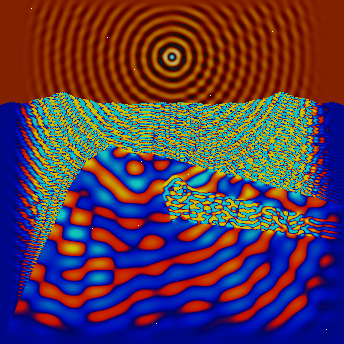
\includegraphics[width=0.8\textwidth]{Images/Automated.png}
		\caption{Algorithm Output for $\omega=100$}
		\label{fig:Automation-small-omega}
	\end{subfigure}%
	\begin{subfigure}{0.5\textwidth}
		\centering
		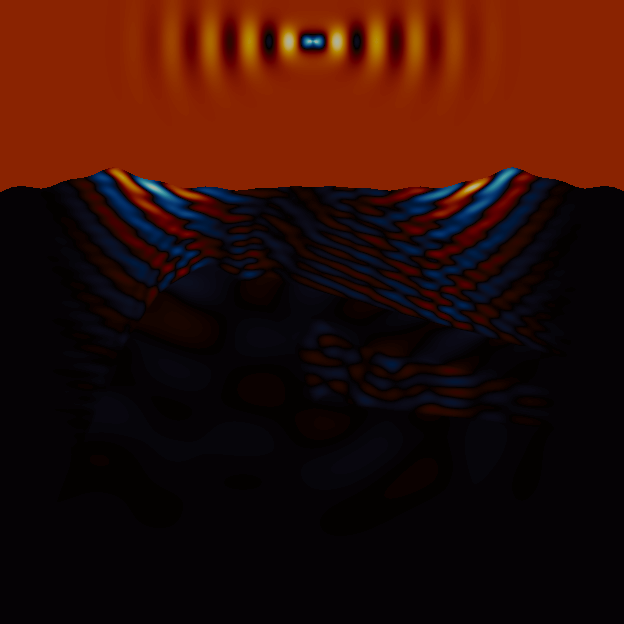
\includegraphics[width=0.8\textwidth]{Images/Automated-Fail.png}
		\caption{Algorithm Output for $\omega=50$}
		\label{fig:Automation-large-omega}
	\end{subfigure}
	\caption{Algorithm Outputs for two angular frequencies}
	\label{fig:Automation-Success-Failure}
\end{figure}


A natural question to ask is whether it is possible to assign a PML only to certain elements in the mesh, not to entire layers around the boundary. Julien Diaz at Magique3D has said that this will cause the PML to be more unstable and will not work, although I have not tested this hypothesis.


\newpage

\subsection{Code [Fortran90]}
\lstset{basicstyle=\small, style=fortranStyle}
\begin{lstlisting}
SUBROUTINE calcPMLCoefficients
    ! written by Andy Wang
    ! currently only works on 2D

    USE PRECISION
    USE constant
    USE mesh
    USE pml
    USE DATA

    IMPLICIT NONE
	
    REAL(kind=dp) :: vp, maxL, lambda
    REAL(kind=dp) :: mult, mlambda      ! mult = L / lambda
    REAL(kind=dp) :: centX, centY
    REAL(kind=dp) :: yb, yt, xl, xr
    REAL(kind=dp) :: dyb, dyt, dxl, dxr
    REAL(kind=dp) :: ndyb, ndyt, ndxl, ndxr
    REAL(kind=dp) :: eps
    INTEGER :: I, II, J, Nodes(3), compte

    mult = 1.5
    eps = 100.

    maxL = -1
    yb = 10000000
    yt = -10000000
    xl = 10000000
    xr = -10000000

    DO I=1,Ntri
        II=ref_media(I)
        IF(acouela(II).EQ.1) THEN
            vp=SQRT(mu_media(II)/rho_media(II))
        ELSE
            vp=SQRT(Cij_media(II,1,1)/rho_media(II))
        ENDIF
        lambda = vp * 2.0 * pi / omega
        mlambda = mult * lambda
        WRITE(6,*) I,vp,omega,lambda,mlambda
        IF (mlambda .GT. maxL) THEN
            maxL = mlambda
        ENDIF
		
        Nodes(:)=Tri(I,:)
        DO J=1,3
            IF (Coor(Nodes(J),1) .LT. xl) THEN
                xl = Coor(Nodes(J),1)
            ENDIF
            IF (Coor(Nodes(J),1) .GT. xr) THEN
                xr = Coor(Nodes(J),1)
            ENDIF
            IF (Coor(Nodes(J),2) .LT. yb) THEN
                yb = Coor(Nodes(J),2)
            ENDIF
            IF (Coor(Nodes(J),2) .GT. yt) THEN
                yt = Coor(Nodes(J),2)
            ENDIF
        ENDDO
    ENDDO

    dyb = maxL
    dyt = maxL
    dxl = maxL
    dxr = maxL

    DO      ! INFINITE LOOP, exiting upon stable condition
            ! in other words:
            ! when projected PML limits at top, bottom, left, right stabilize
        ndyb = -1
        ndyt = -1
        ndxl = -1
        ndxr = -1

        DO I=1,Ntri
            Nodes(:)=Tri(I,:)
            centX = 0
            centY = 0    ! represent the coordinates of the centroid
            DO J=1,3
                centX = centX + Coor(Nodes(J),1)
                centY = centY + Coor(Nodes(J),2)
            ENDDO
            centX = centX / 3
            centY = centY / 3

            II=ref_media(I)
            IF(acouela(II).EQ.1) THEN
                vp=SQRT(mu_media(II)/rho_media(II))
            ELSE
                vp=SQRT(Cij_media(II,1,1)/rho_media(II))
            ENDIF
            lambda = vp * 2.0 * pi / omega
            mlambda = mult * lambda

            IF (centY .LT. yb + dyb) THEN   ! if it's in the bottom PML
                IF (mlambda .GT. ndyb) THEN
                    ndyb = mlambda
                ENDIF
            ENDIF
            IF (centY .GT. yt - dyt) THEN   ! if it's in the top PML
                IF (mlambda .GT. ndyt) THEN
                    ndyt = mlambda
                ENDIF
            ENDIF
            IF (centX .LT. xl + dxl) THEN   ! if it's in the left PML
                IF (mlambda .GT. ndxl) THEN
                    ndxl = mlambda
                ENDIF
            ENDIF
            IF (centX .GT. xr - dxr) THEN   ! if it's in the right PML
                IF (mlambda .GT. ndxr) THEN
                    ndxr = mlambda
                ENDIF
            ENDIF
        ENDDO

        IF ((dyb-ndyb) + (dyt-ndyt) + (dxl-ndxl) + (dxr-ndxr) .LT. eps) THEN
            dyb = ndyb
            dyt = ndyt
            dxl = ndxl
            dxr = ndxr
            EXIT		
        ENDIF
        dyb = ndyb
        dyt = ndyt
        dxl = ndxl
        dxr = ndxr
    ENDDO

    pmlayer%yb = yb + ndyb
    pmlayer%yt = yt - ndyt
    pmlayer%xl = xl + ndxl
    pmlayer%xr = xr - ndxr

    CALL calcZetaCoefficient(pmlayer%coeff_b, ndyb)
    CALL calcZetaCoefficient(pmlayer%coeff_t, ndyt)
    CALL calcZetaCoefficient(pmlayer%coeff_l, ndxl)
    CALL calcZetaCoefficient(pmlayer%coeff_r, ndxr)
    
    CONTAINS
        SUBROUTINE calcZetaCoefficient(var, delta)
            REAL(kind=dp) :: delta, c, R, var
            R = 0.001       ! as defined in "analyse de stabilite" (96)
            c = delta * omega / (2 * pi * mult)
            var = (3 * c) / (2 * (delta ** 3)) * LOG(1 / R)
        END SUBROUTINE calcZetaCoefficient
        
END SUBROUTINE calcPMLCoefficients
\end{lstlisting}

